\section{Modello ISO-OSI}
\subsection{Introduzione}
Il modello ISO-OSI è un modello di riferimento per la progettazione e l'implementazione di reti di telecomunicazioni. È stato sviluppato dall'Organizzazione Internazionale per la Standardizzazione (ISO) negli anni '80 e fornisce un framework concettuale per comprendere come i diversi protocolli e tecnologie di rete interagiscono tra loro.

ISO OSI non ha un numero fisso di livelli, è importante capire la logica dei livelli che devono comporre un modello iso osi ma il numero specifico dei livelli può variare a seconda della necessità.

Il modello più comune di ISO-OSI è composto da sette livelli, ognuno dei quali svolge funzioni specifiche e comunica con i livelli superiori e inferiori. I sette livelli sono:
\begin{enumerate}
    \item \textbf{Livello fisico}: si occupa della trasmissione dei dati attraverso il mezzo fisico (cavi, fibre ottiche, onde radio, ecc.). Definisce le caratteristiche elettriche e meccaniche dei dispositivi di rete.
    \item \textbf{Livello di collegamento dati}: gestisce la comunicazione tra i dispositivi sulla stessa rete locale. Si occupa della rilevazione e correzione degli errori, del controllo del flusso e dell'indirizzamento fisico (MAC).
    \item \textbf{Livello di rete}: si occupa dell'instradamento dei pacchetti tra reti diverse. Utilizza indirizzi logici (come gli indirizzi IP) per identificare i dispositivi sulla rete e determina il percorso migliore per inviare i dati.
    \item \textbf{Livello di trasporto}: garantisce la consegna affidabile dei dati tra i dispositivi. Si occupa della segmentazione dei dati, del controllo degli errori e del controllo del flusso. I protocolli più comuni a questo livello sono TCP e UDP.
    \item \textbf{Livello di sessione}: gestisce le sessioni di comunicazione tra i dispositivi. Si occupa dell'apertura, della chiusura e del mantenimento delle sessioni, nonché della sincronizzazione dei dati.
    \item \textbf{Livello di presentazione}: si occupa della formattazione e della codifica dei dati. Converte i dati in un formato comprensibile per il livello applicativo e gestisce la compressione e la crittografia dei dati.
    \item \textbf{Livello applicativo}: è il livello più alto del modello e fornisce servizi di rete agli utenti finali. Include protocolli come HTTP, FTP, SMTP e DNS, che consentono la comunicazione tra applicazioni.
\end{enumerate}

\begin{figure}[h!]
    \centering
    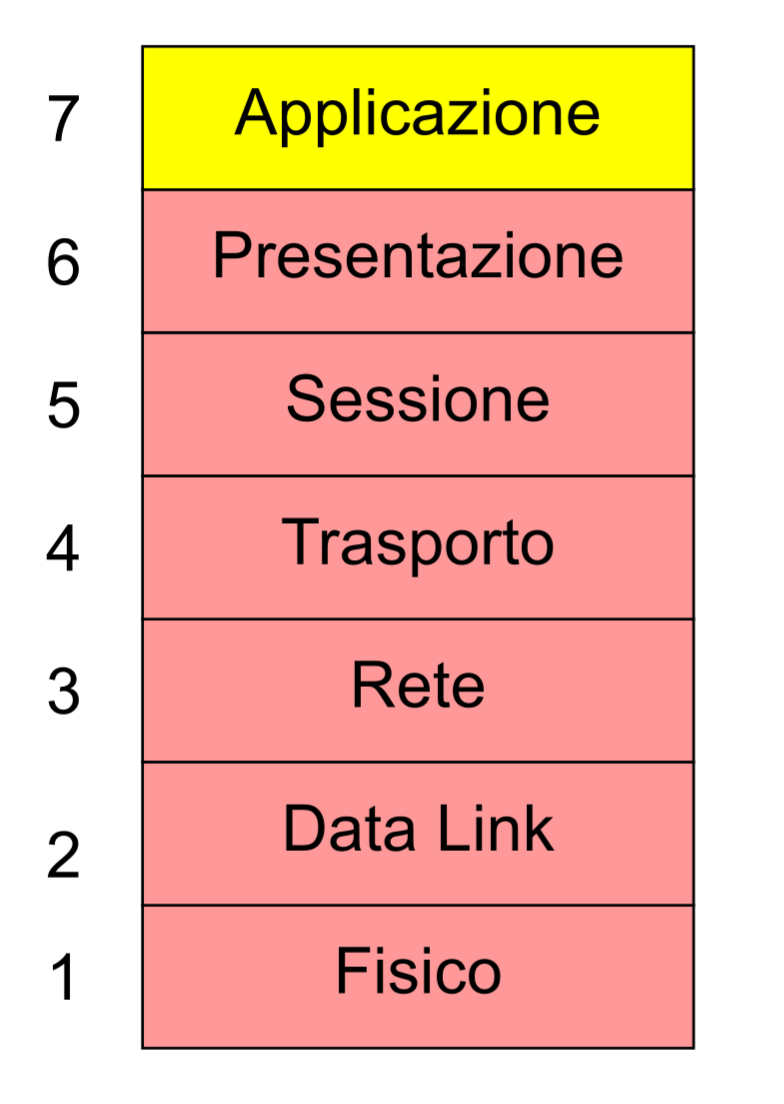
\includegraphics[width=0.45\textwidth]{images/ISO_OSI_livelli.png}
    \caption{I sette livelli del modello ISO-OSI}
    \label{fig:iso_osi_livelli}
\end{figure}

L'ISO-OSI serve a descrivere l'architettura dei protocolli, tramite il raggruppamento e la stratificazione.
vengono raggruppate tra loro le funzioni simili per logica o tecnologia.
questi gruppi vengono organizzati in modo gerarchico, quindi a strati(stratificazione). con ogni strato ci si può interfacciare trazie alle interfacce.
lo strato N è costituito da una o più entità e l'interazione tra due sistemi avviene tra strati di eguale livello e con entità pari.

Con il modello iso osi i “problemi” nella progettazione vengono divisi, rendendo la progettazione più modulare e più semplice, potendo specializzarsi su un livello specifico del modello. dividere un problema in più livelli è più conveniente. 
\subsubsection{Entità e pacchetti}
Ogni livello ha un'entità, queste elaborano i pacchetti, un pacchetto(PDU: protocol data unit) è composto da un header(PCI:protocol control information) e un payload(SDU: service data unit) 
\subsection{Segmentazione e riassemblaggio} 
La segmentazione è il processo di suddivisione dei dati in pacchetti più piccoli per facilitarne la trasmissione attraverso la rete. Ogni pacchetto viene inviato separatamente e può seguire percorsi diversi attraverso la rete. Il riassemblaggio è il processo inverso, in cui i pacchetti ricevuti vengono ricomposti nell'ordine corretto per ricostruire i dati originali.
(dall’alto verso il basso(segmentazione) vengono aggiunti gli header ai pacchetti; dal basso verso l’alto(riassemblaggio) vengono rimossi, quindi utilizzati, gli header dei pacchetti)
\subsubsection{Incapsulamento e decapsulamento}
Dall'alto verso il basso: trasmissione $\rightarrow$ da tenere a mente che il livello più basso c’è il livello fisico, mentre il livello più alto è quello a cui tipicamente ci interfacciamo(applicazione del telefono ad esempio, whatsapp)
quando trasmetto quindi faccio encapsulation, ossia aggiungo informazioni utili alla trasmissione del payload. questo perchè tra un livello è l’altro potrei avere la necessità di dover dividere il pacchetto in altri pacchetti, perciò va aggiunto negli header le informazioni necessarie a far riassemblare il pacchetto intero una volta finita la trasmissione.
\begin{figure}[h!]
    \centering
    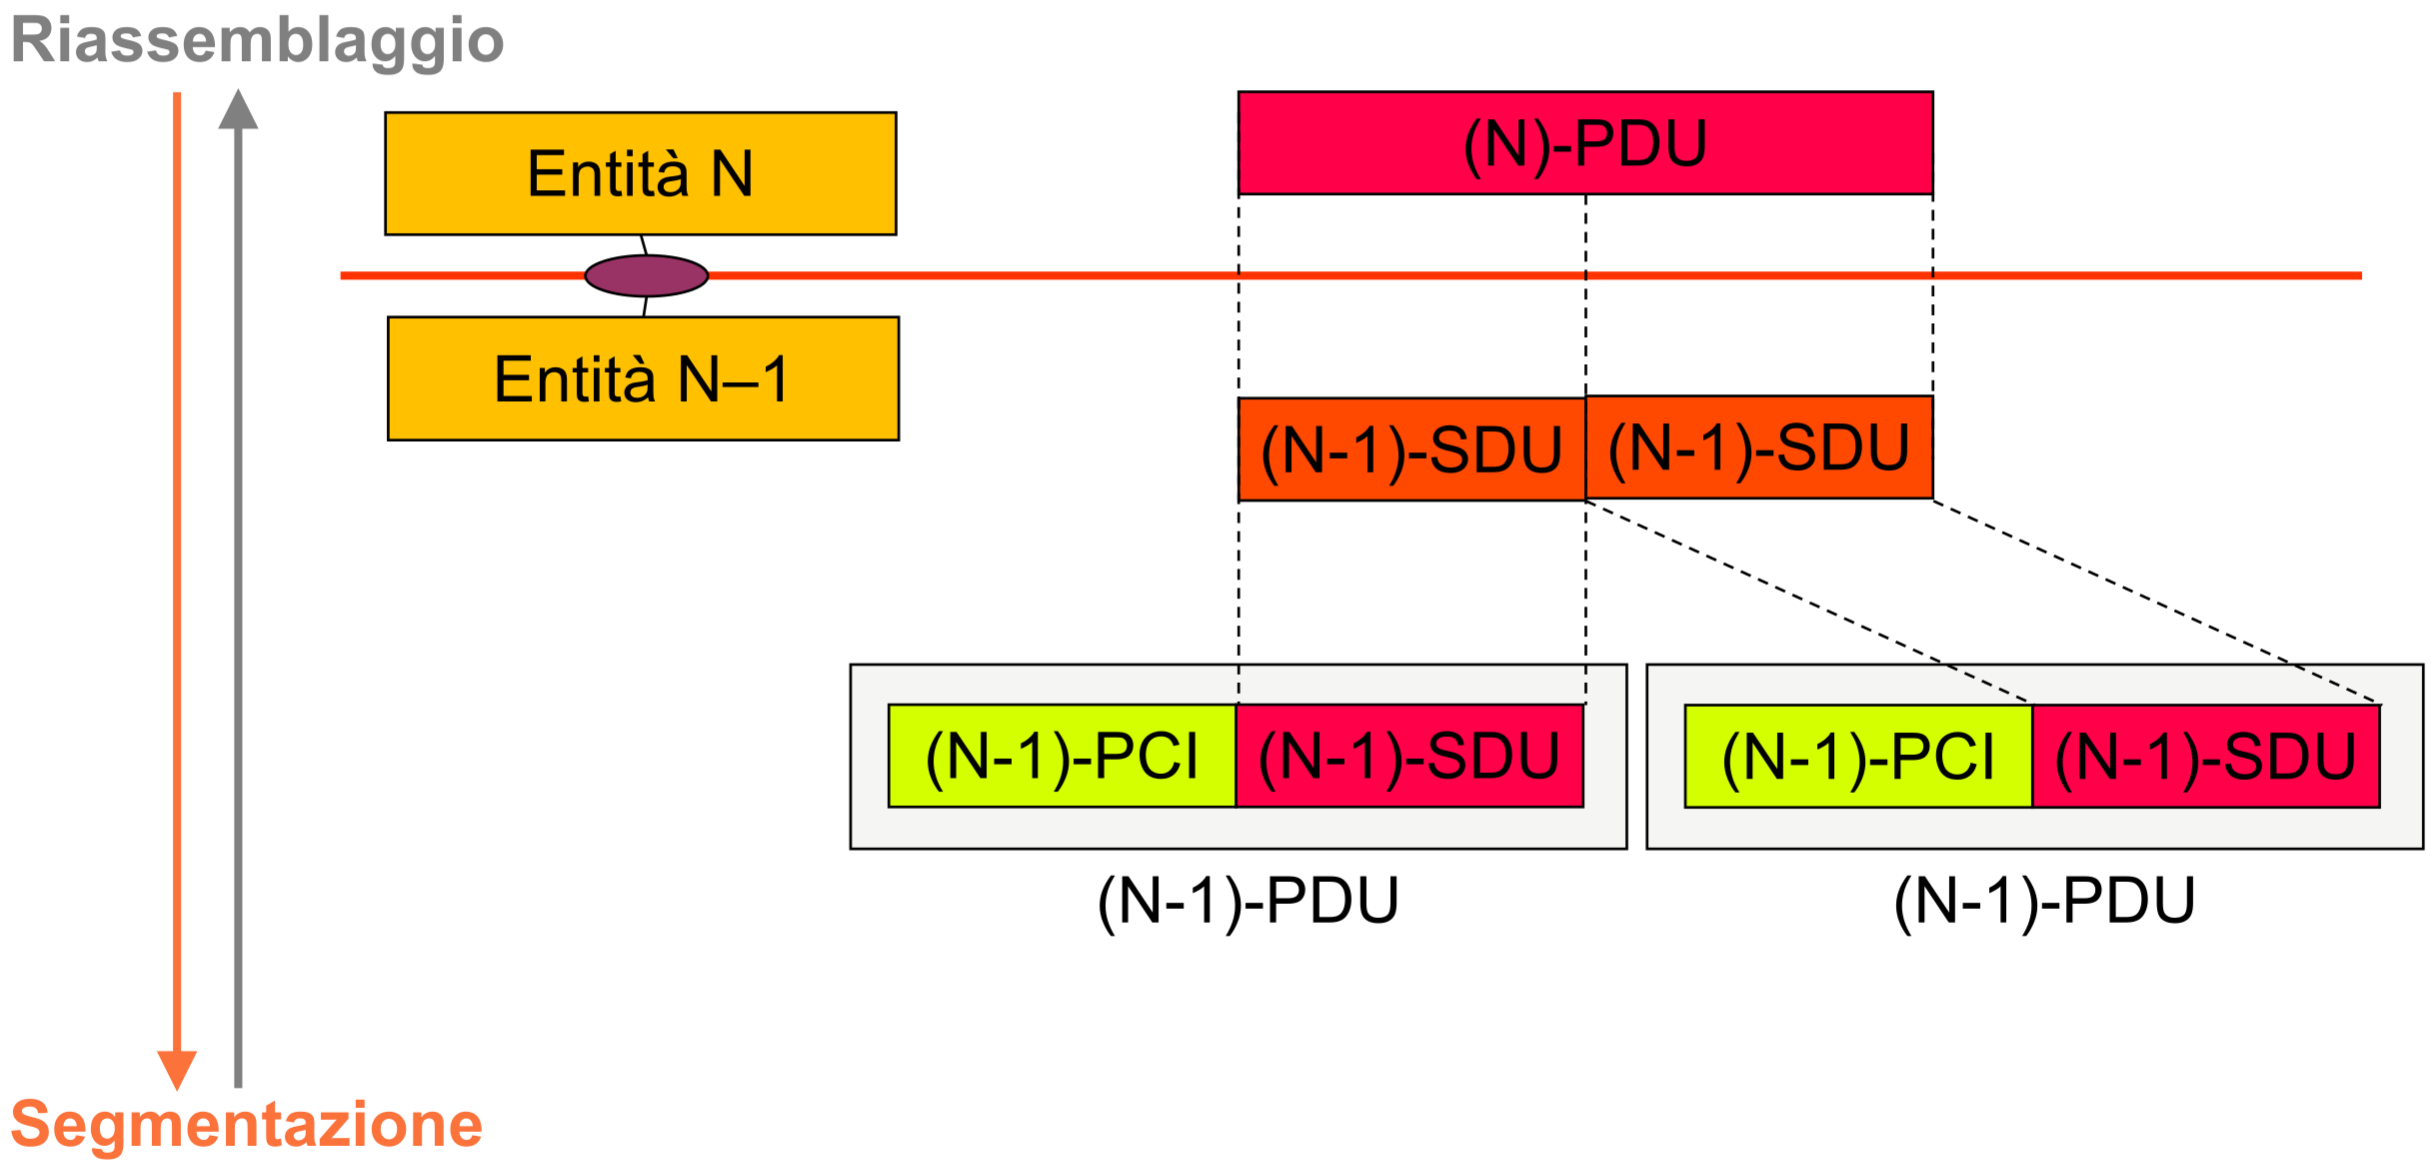
\includegraphics[width=1\textwidth]{images/ISO_OSI_incapsulamento.png}
    \caption{Pacchetti e incapsulamento/decapsulamento}
    \label{fig:pacchetti}
\end{figure}



\newpage
\section{Modello ibrido}
Il modello ibrido è un modello di rete che combina elementi del modello ISO-OSI e del modello TCP/IP. È stato sviluppato per affrontare le limitazioni del modello ISO-OSI e per adattarsi meglio alle esigenze delle reti moderne.
Il modello ibrido è composto da cinque livelli principali:
\begin{enumerate}
    \item \textbf{Livello fisico}: simile al livello fisico del modello ISO-OSI, si occupa della trasmissione dei dati attraverso il mezzo fisico.
    \item \textbf{Livello di collegamento dati}: gestisce la comunicazione tra i dispositivi sulla stessa rete locale e include funzioni di rilevamento degli errori e controllo del flusso.
    \item \textbf{Livello di rete}: simile al livello di rete del modello ISO-OSI, si occupa dell'instradamento dei pacchetti tra reti diverse.
    \item \textbf{Livello di trasporto}: fornisce servizi di trasporto affidabili e non affidabili, come TCP e UDP.
    \item \textbf{Livello applicativo}: fornisce servizi di rete agli utenti finali e include protocolli come HTTP, FTP e SMTP.
    \end{enumerate}

    \begin{figure}[h!]
    \centering
    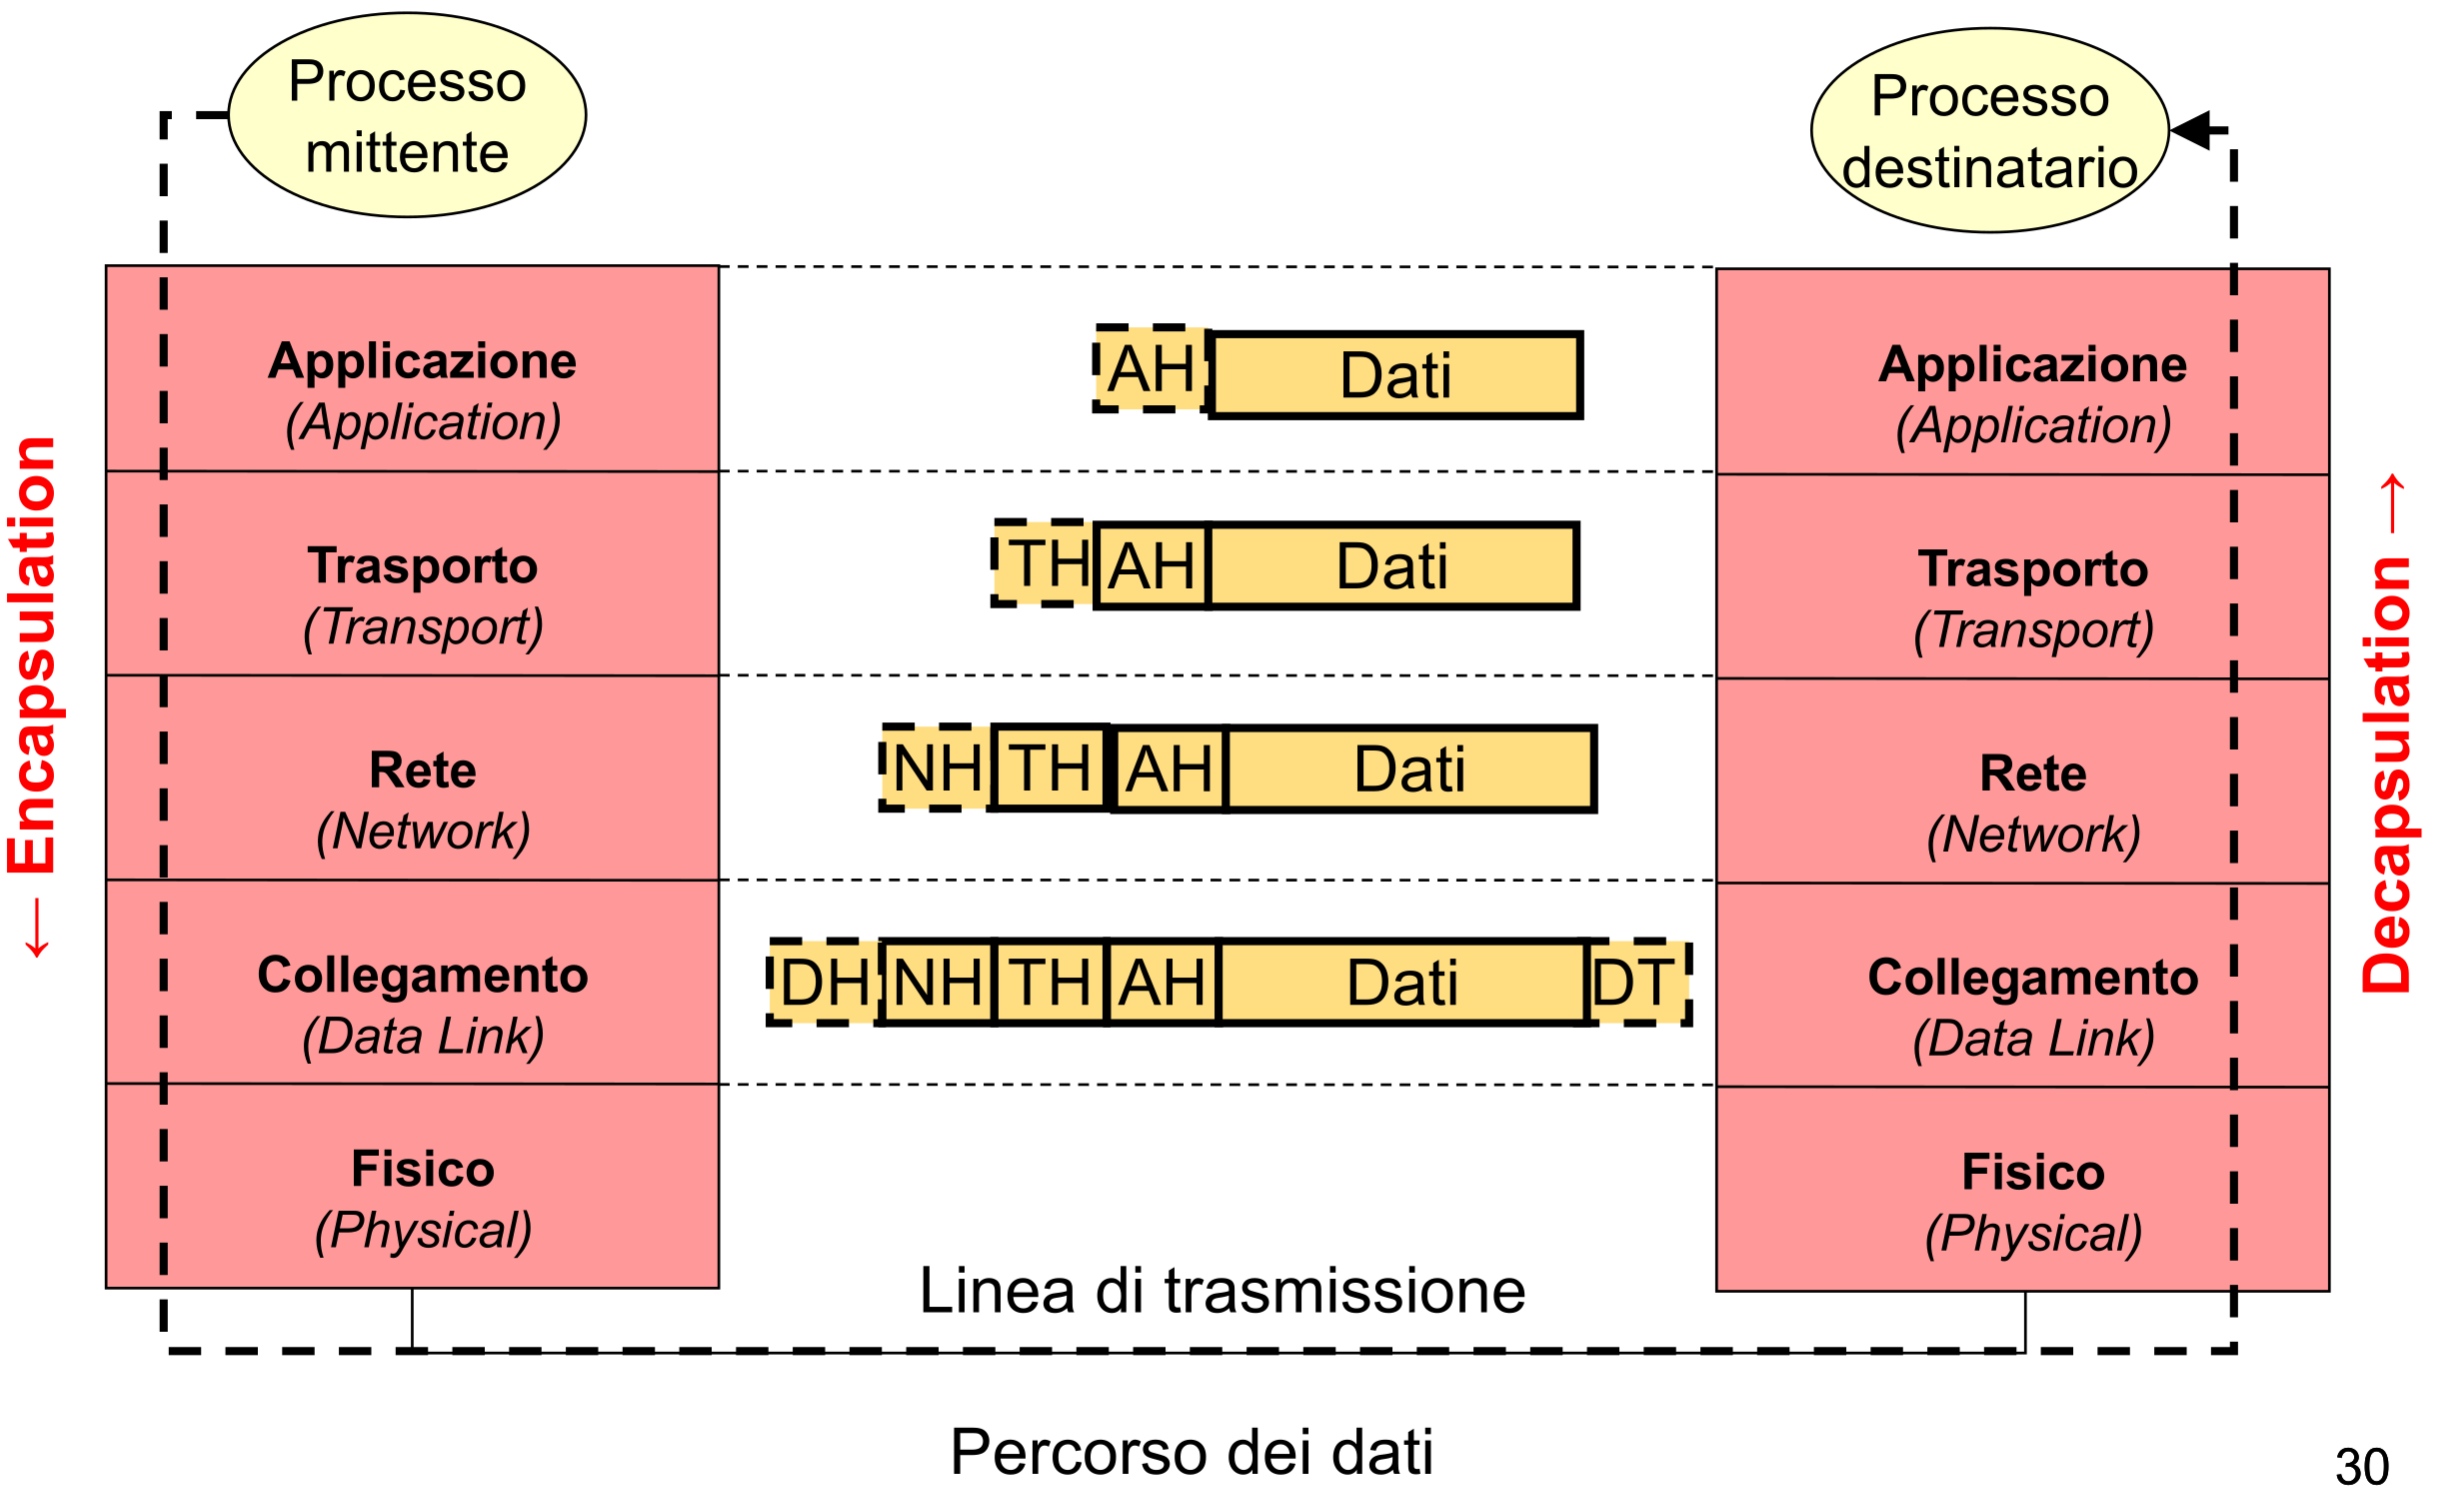
\includegraphics[width=1.2\textwidth]{images/enc_dec_ibrido.png}
    \caption{Incapsulamento e decapsulamento dei dati nel modello ibrido}
    \label{fig:modello_ibrido_enc_decapsulamento}
\end{figure}

\subsection{Enc/decapsulation dati nel modello ibrido}
Durante l'encapsulation vengono ad ogni livello aggiunti degli header(AH = application heder, TH = transport header, NH = network header ecc), durante la decapsulation vengono spacchettati grazie agli header precedentemente aggiunti ad ogni livello
l'unico livello che aggiunge oltre ad un header anche una coda(tail) è il “data link” , “collegamento”, questo perchè vuole verificare la correttezza del pacchetto, tramite tecniche che vedrò avanti(algoritmi di controllo, non esiste un metodo che garantisce che il pacchetto che sia 100% corretto, come l’evenienza in cui dopo la verifica mi risulta corretto ma poi si scopre incorretto, falso positivo).

\subsection{Comunicazione tra sistemi}
i livelli rete, data link e fisico si occupano del trasporto dell’informazione tra il sistema a ed il sistema b. questo può avvenire tramite il nodi, intermediari, x e y, oppure in modo diretto.
il datalink presuppone un collegamento diretto ed è fondamentale che riceva informazion dal livello fisico poichè gestisce il passaggio di info tra un mezzo fisico e l’altro. al pacchetto viene aggiunto tramite il datalink un header che gestisce il passaggio tra a e x, quindi utilizzando un indirizzo locale. a livello di datalink inoltre viene viene verificato che il pacchetto sia inviato correttamente(evitando il loop: deadlog). dopo aver verificato la correttezza del pacchetto, a livello di rete ci si assicura che il pacchetto ricevuto sia arrivato a destinazione. nel caso specifico il pacchetto che arriva al livello di rete del nodo x viene spedito al nodo successivo poichè il livello di rete del nodo x capisce che non era lui il destinatario, tramite la lettura dell’header inserito dal sistema a inizialmente. 
tra un nodo e l’altro è possibile usare tecnologie differenti, cavo, wireless ecc, livello fisico

se al livello b arriva un pacchetto errato allora viene reinviato il pacchetto da b ad a così da far capire ad a che deve reinviare il pacchetto, latenza.
posso inserire un timer oltre il quale si interrompe la trasmissione, per evitare loop o perdite di informazioni.

\begin{figure}[h!]
    \centering
    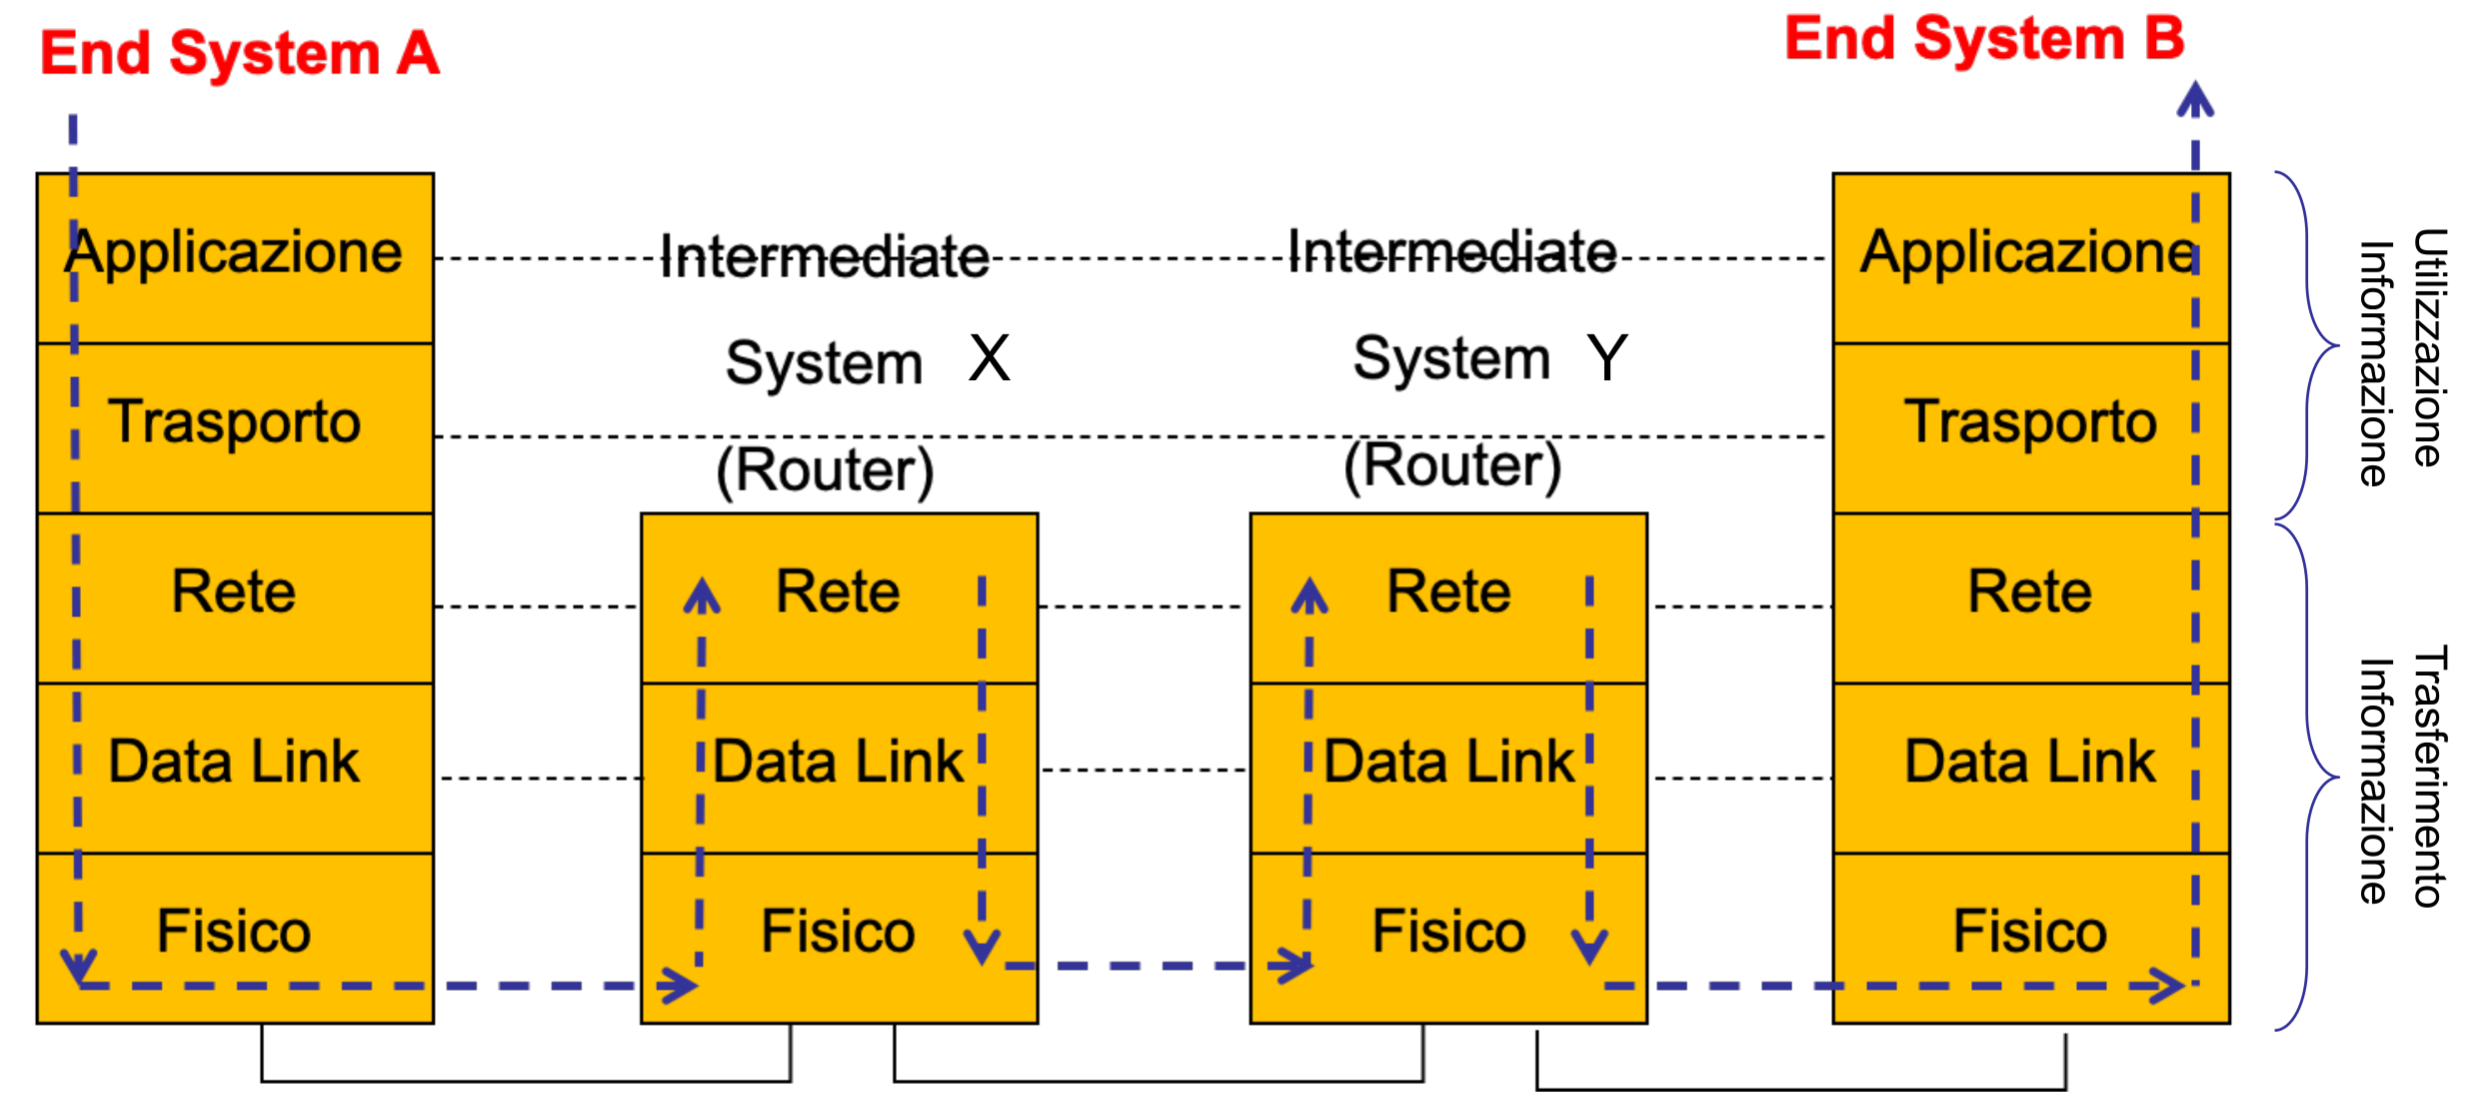
\includegraphics[width=1\textwidth]{images/comunicazione_ibrido.png}
    \caption{Comunicazione tra sistemi nel modello ibrido}
    \label{fig:comunicazione_sistemi_ibrido}
\end{figure}


    \newpage
\section{Modello TCP/IP}
Il modello tcp/ip nasce a 4 livelli, il livelllo di rete si chiama internet, poichè a quel livello si usa il protocollo ip(internet protocol).





\begin{figure}[h!]
    \centering
    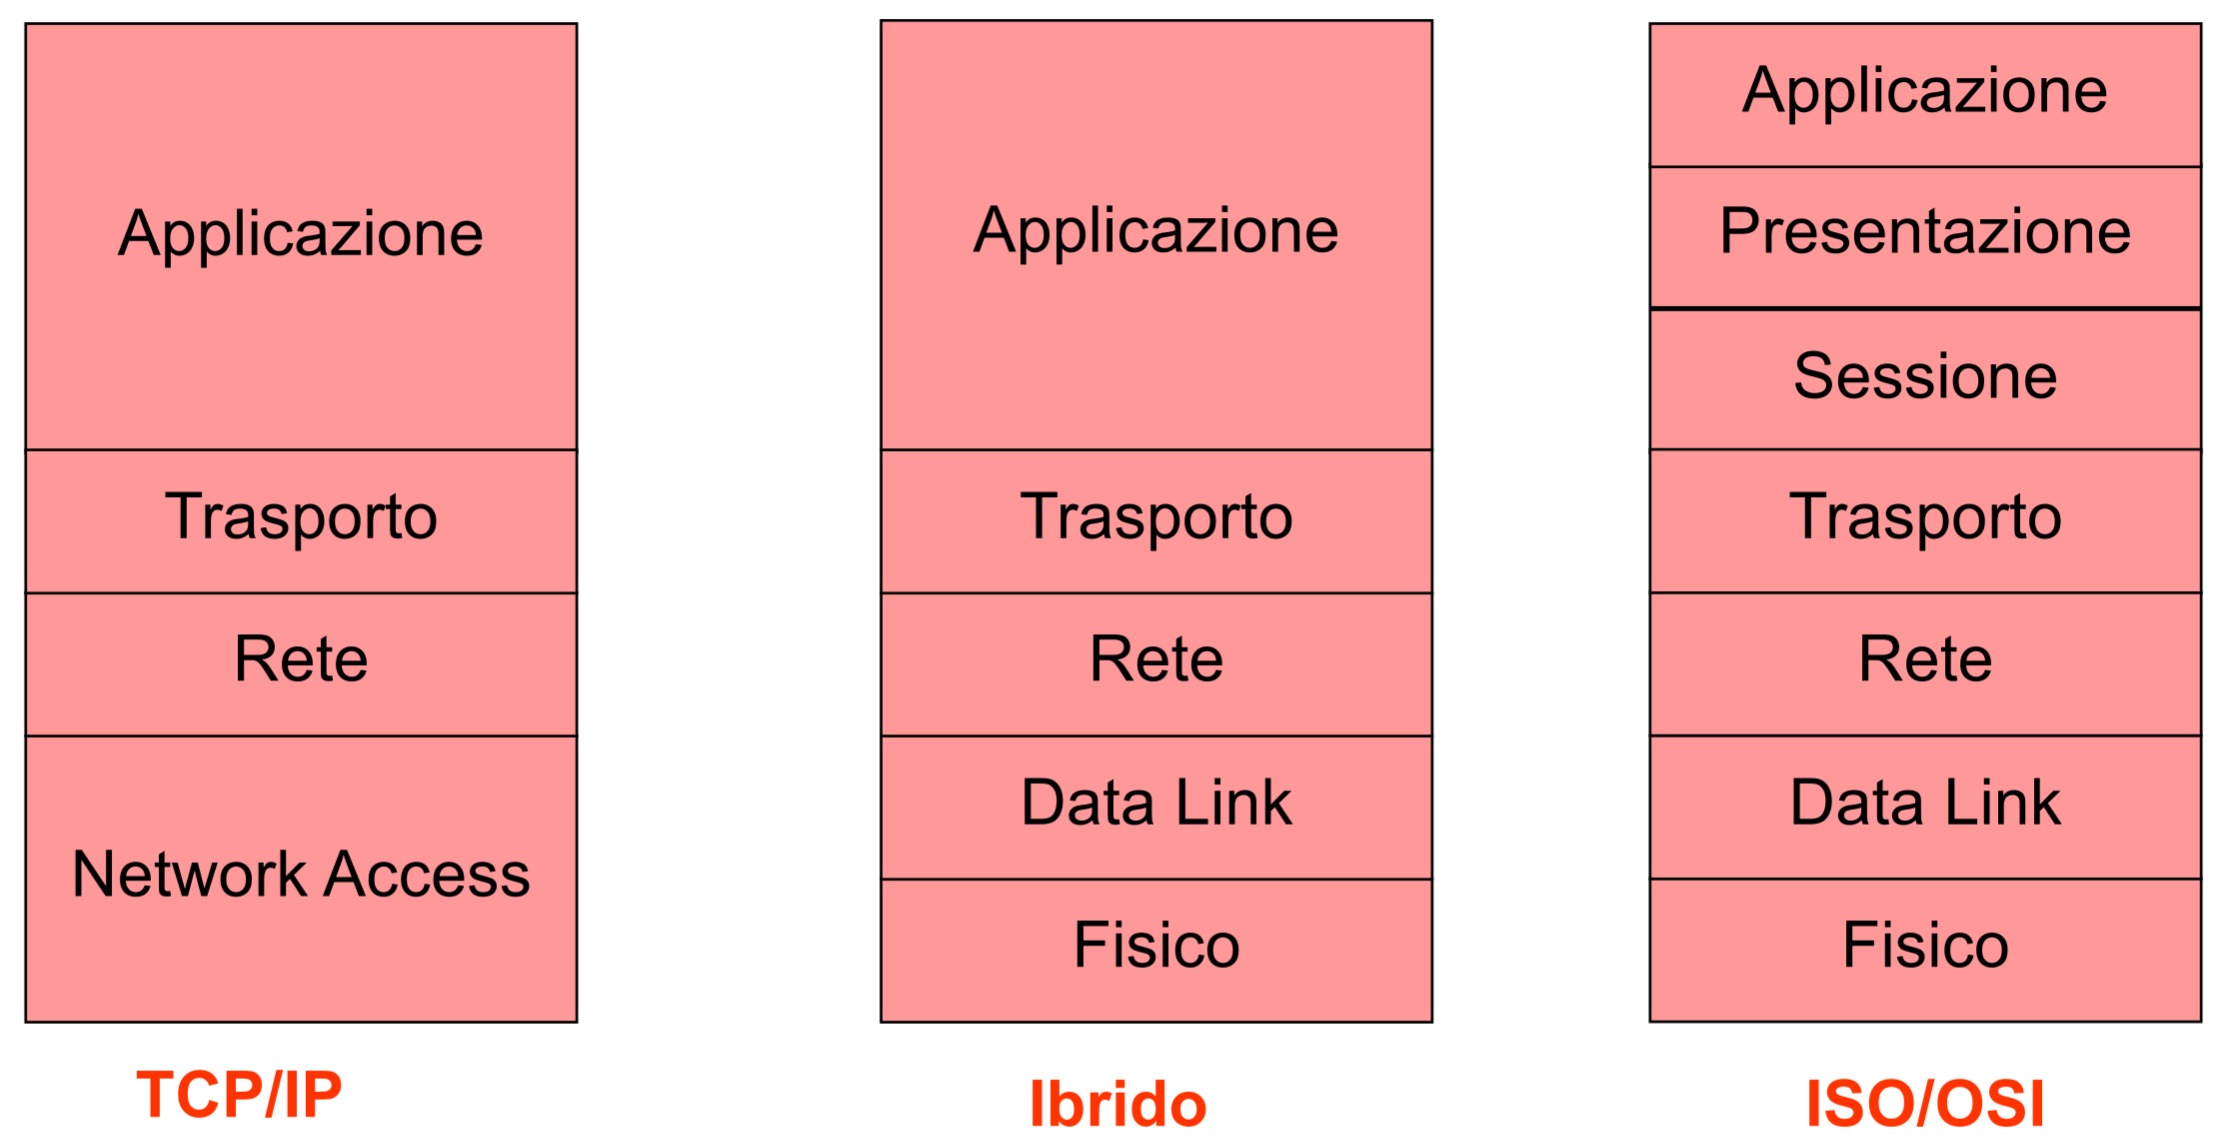
\includegraphics[width=1\textwidth]{images/confronto_stack.png}
    \caption{Confronto tra stack ISO-OSI, TCP/IP e modello ibrido}
    \label{fig:confronto_stack}
\end{figure}